\documentclass[11pt,a4paper]{article}

%% ---------------------------------------------------------------- packages
\usepackage[utf8]{inputenc}
\usepackage[T1]{fontenc}
\usepackage[english]{babel}
\usepackage[a4paper,margin=2cm]{geometry}
\usepackage{amsmath,amssymb}
\usepackage{graphicx}
\usepackage{caption}
\usepackage{float}

\captionsetup{font=small, labelfont=bf}
\setlength{\parindent}{0pt}
\pagestyle{empty}

\begin{document}

%% ================================================================ TITLE
\begin{center}
{\Large\bfseries Flow over an airfoil\par}
\vspace{0.6em}
{\normalsize Ismael Mart\'in D\'iez\par}
\vspace{0.1em}
{\small Engineering Fluid Mechanics --- Aerospace Engineering, Universidad Carlos III de Madrid\par}
\vspace{0.1em}
{\small November 22, 2026\par}
\end{center}
\vspace{-0.3em}
\rule{\linewidth}{0.4pt}
\vspace{0.6em}

%% The guidelines ask for six labelled plots with a brief caption each and no further discussion.
%% NACA 2410, c = 1 m, U = 10 m/s, Spalart-Allmaras; figures 1-4 at alpha = 6 deg.

\begin{figure}[H]
\centering
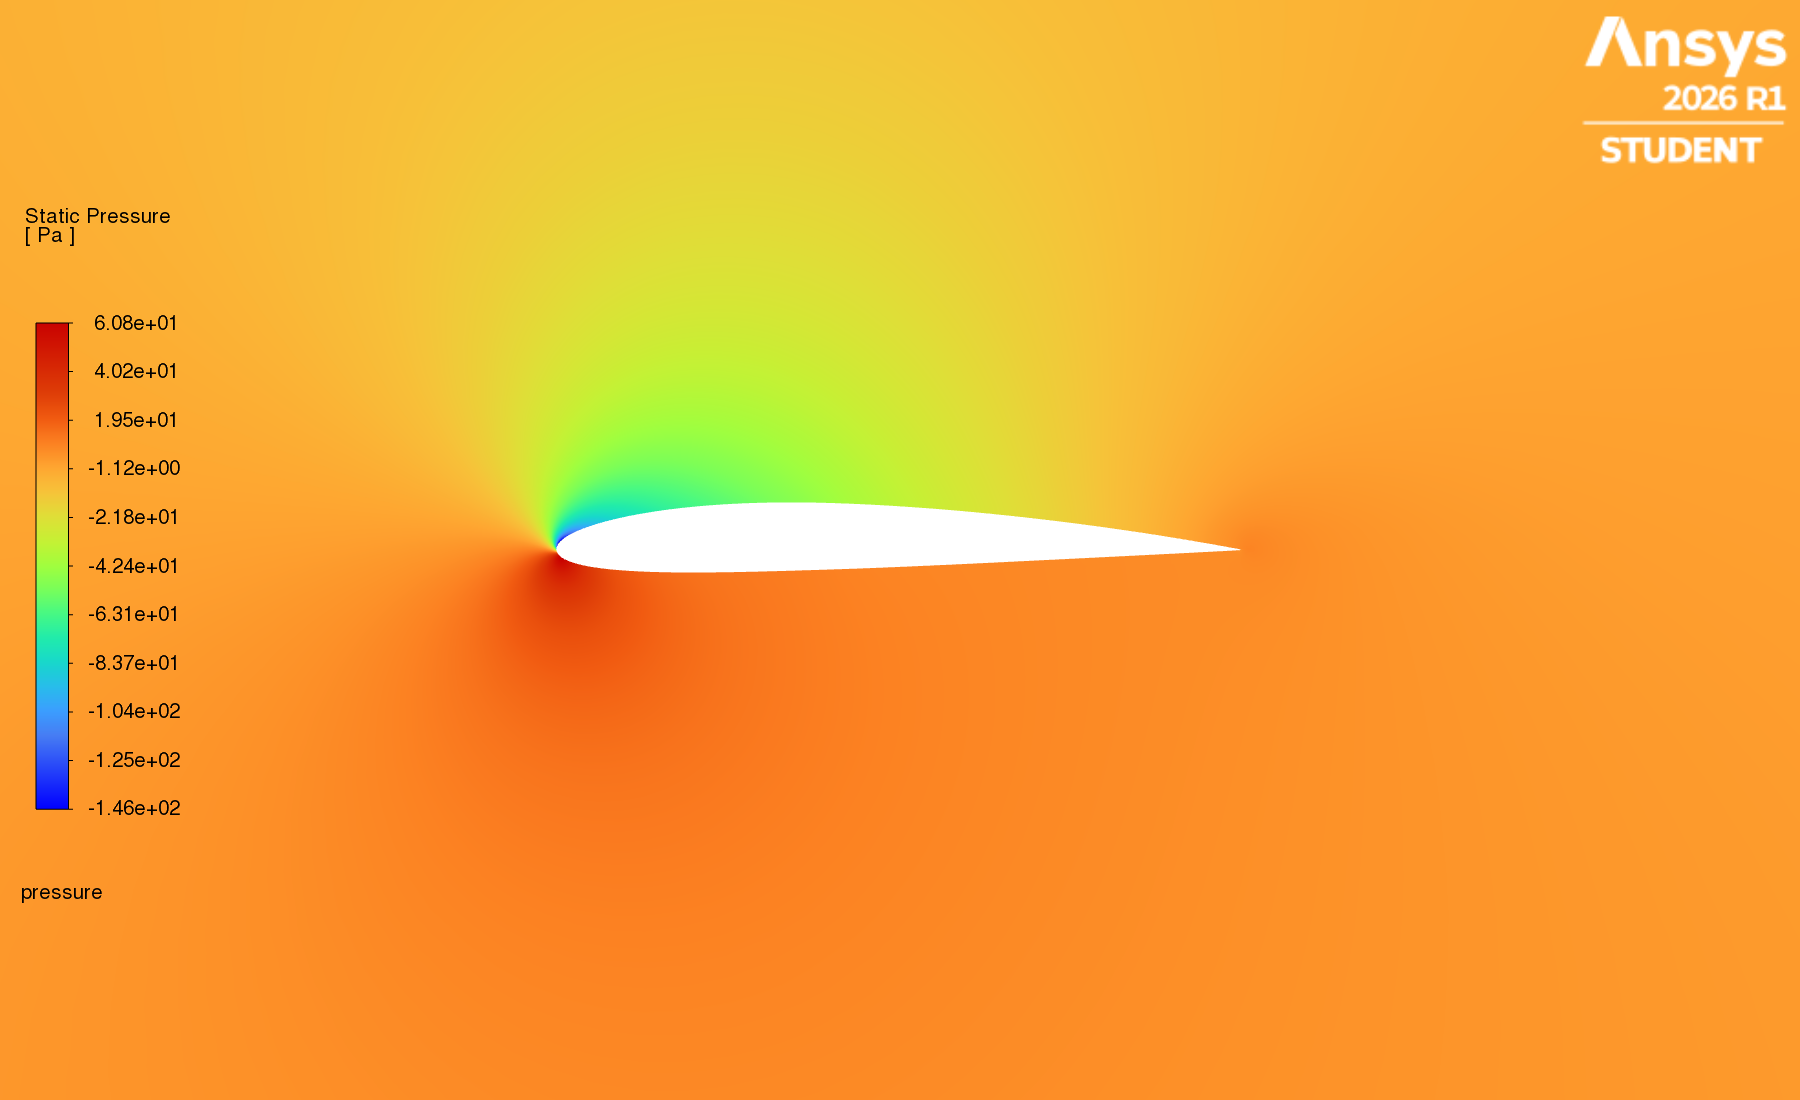
\includegraphics[width=0.85\linewidth]{fig1_pressure_aoa6.png}
\caption{Static pressure around the NACA 2410 airfoil at $\alpha=6^\circ$ ($U=10$~m/s, $c=1$~m). The highest pressure ($61$~Pa) is at the stagnation point, just below the leading edge, and the lowest ($-146$~Pa) is on the upper surface right behind it. The top of the airfoil ends up below ambient pressure and the bottom above it, and that difference is what holds it up.}
\label{fig:pressure}
\end{figure}

\begin{figure}[H]
\centering
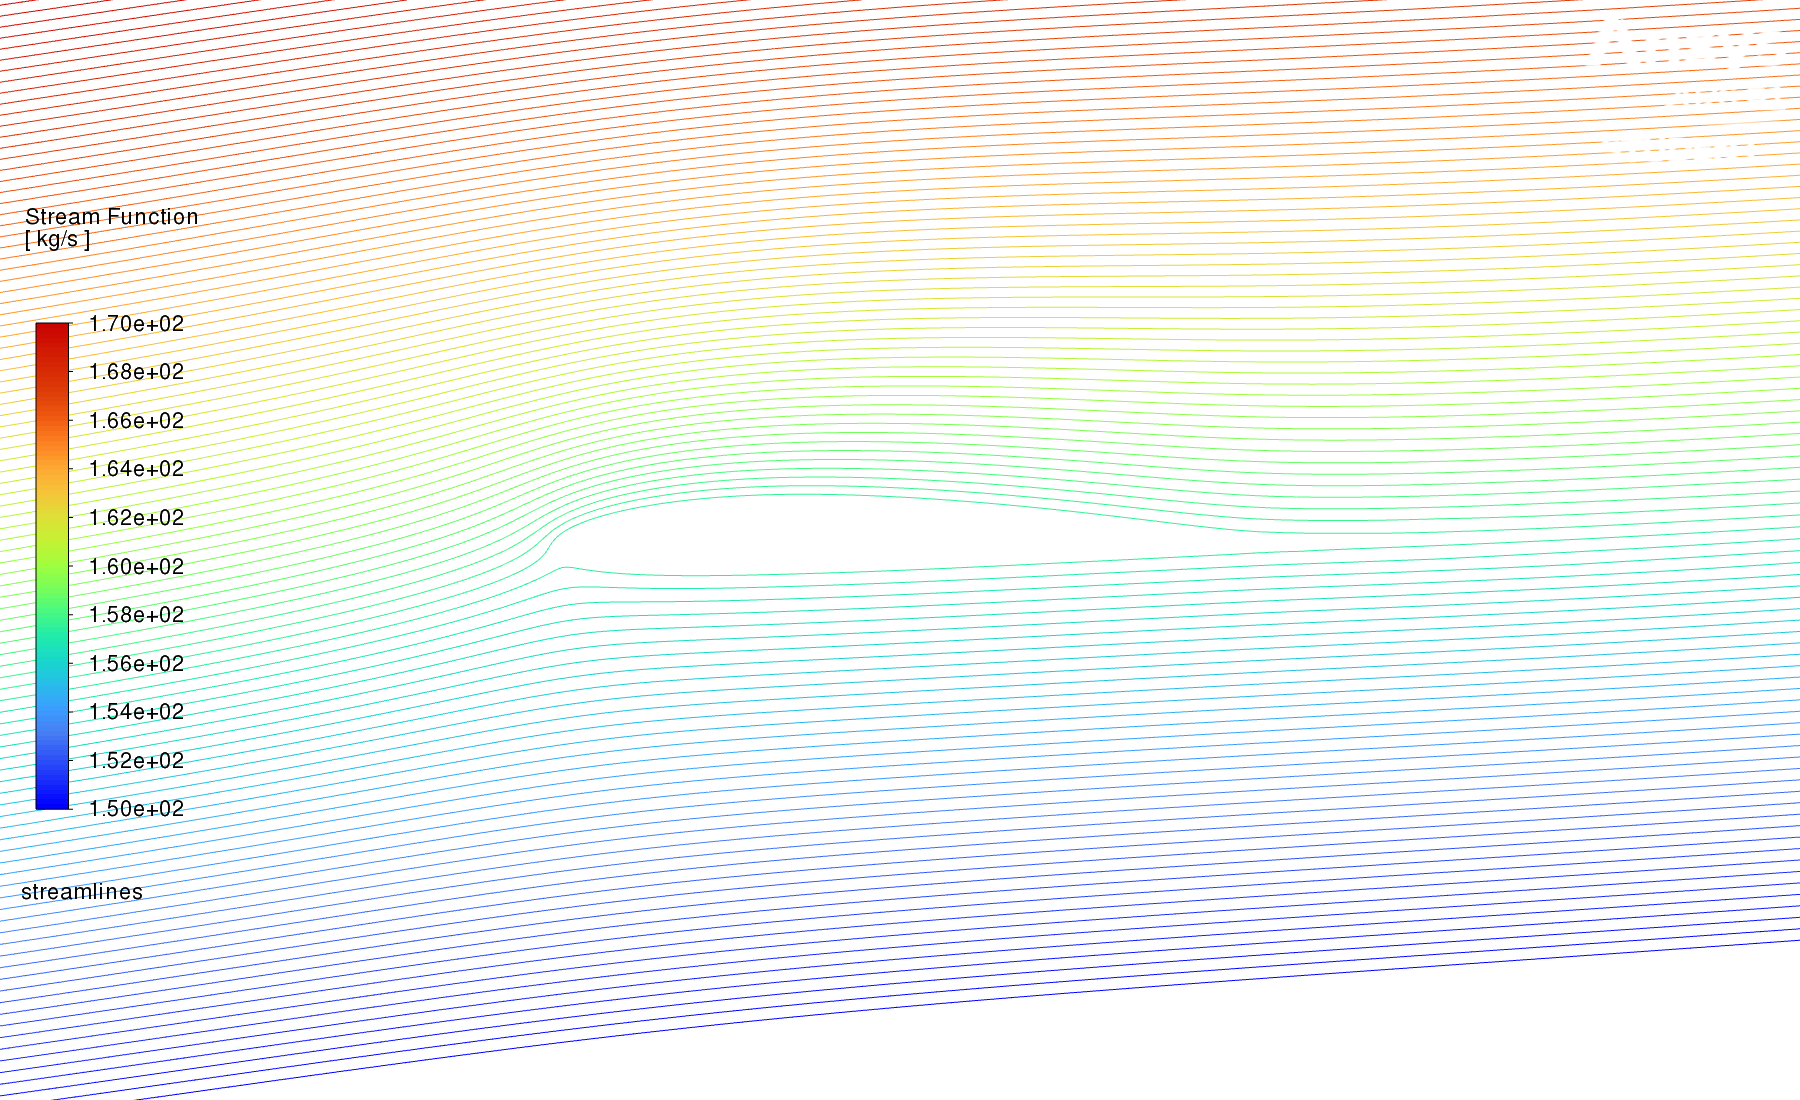
\includegraphics[width=0.85\linewidth]{fig2_streamlines_aoa6.png}
\caption{Streamlines at $\alpha=6^\circ$ (stream function contours between $150$ and $170$~kg/s). The flow splits at the stagnation point under the leading edge. Over the upper surface the lines get closer together, which means the air is going faster there.}
\label{fig:streamlines}
\end{figure}

\begin{figure}[H]
\centering
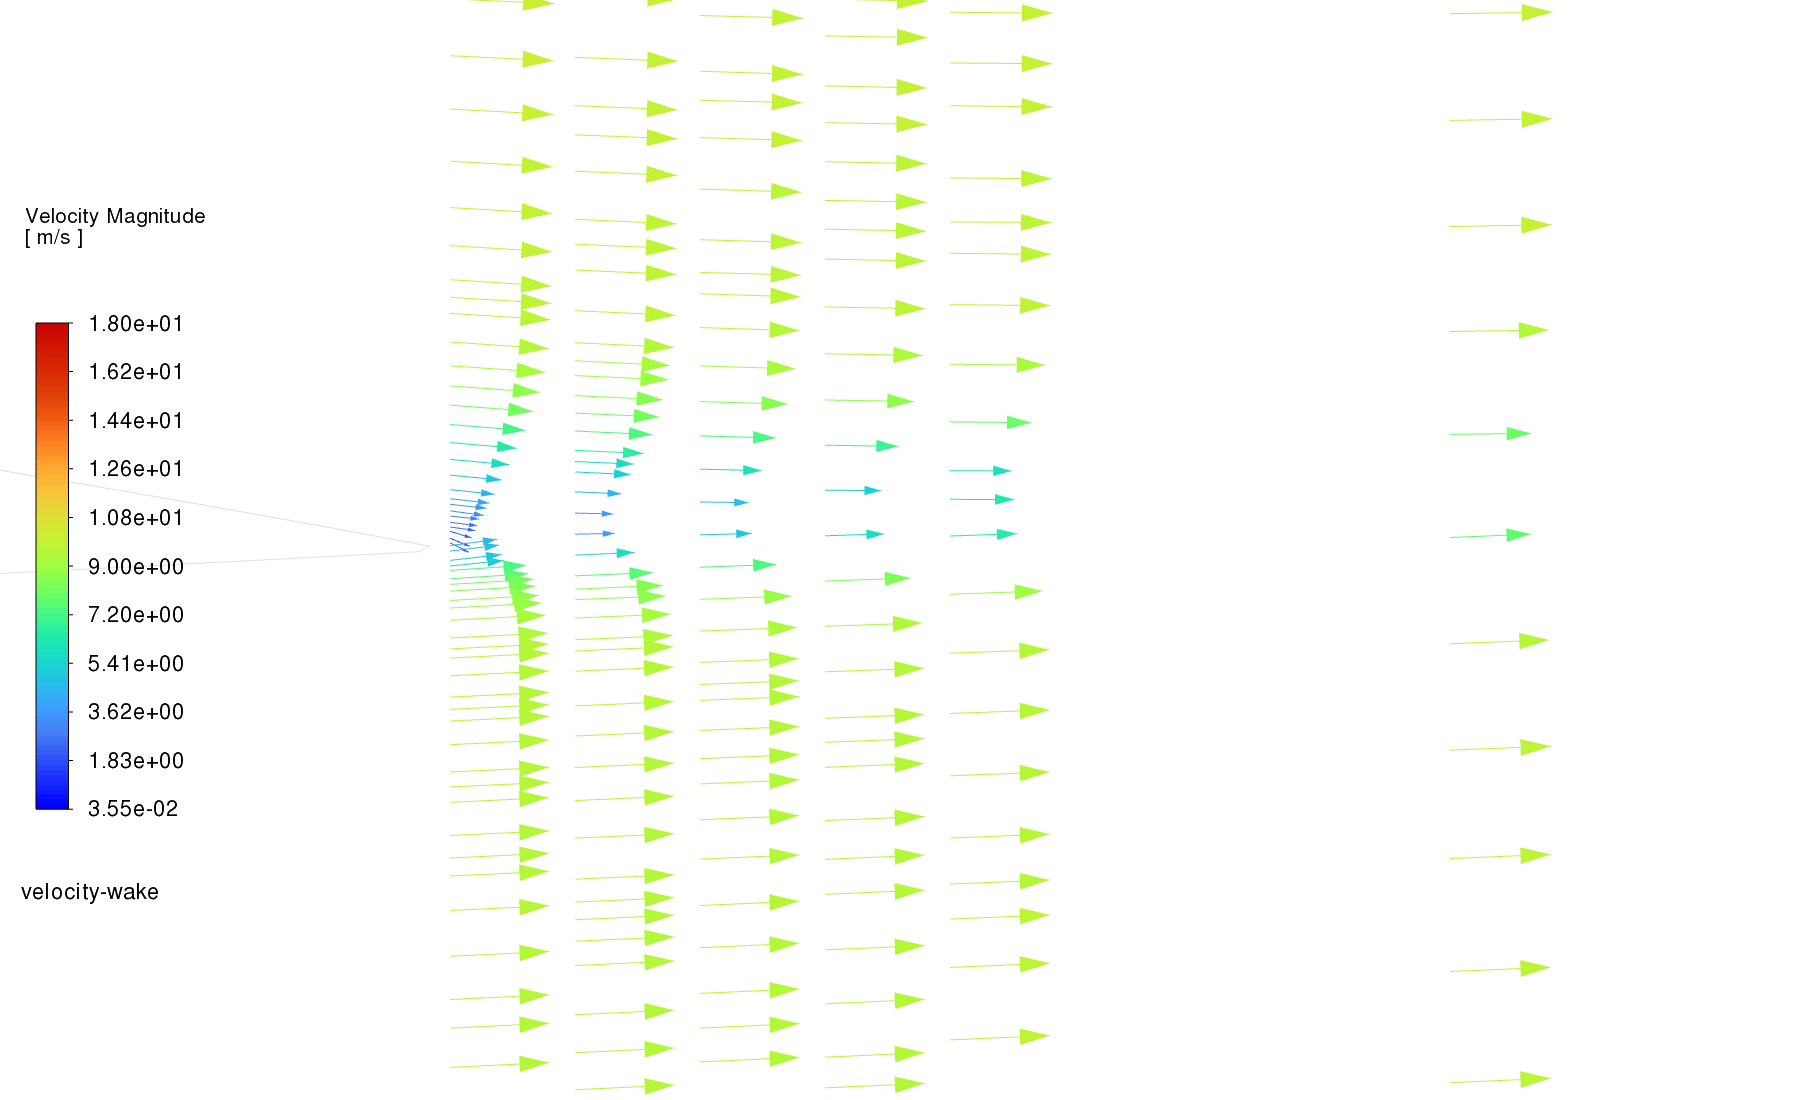
\includegraphics[width=0.85\linewidth]{fig3_quiver_wake_aoa6.png}
\caption{Velocity vectors in the near wake at $\alpha=6^\circ$, on vertical lines at $x=1.0$, $1.025$, $1.05$, $1.075$, $1.1$ and $1.2$~m (trailing edge at $x\simeq1$~m), coloured by velocity magnitude. Right behind the trailing edge the arrows near $y\simeq0$ are much shorter, because friction on the airfoil has slowed that air down. Further downstream this gap in velocity fills in again.}
\label{fig:wake}
\end{figure}

\begin{figure}[H]
\centering
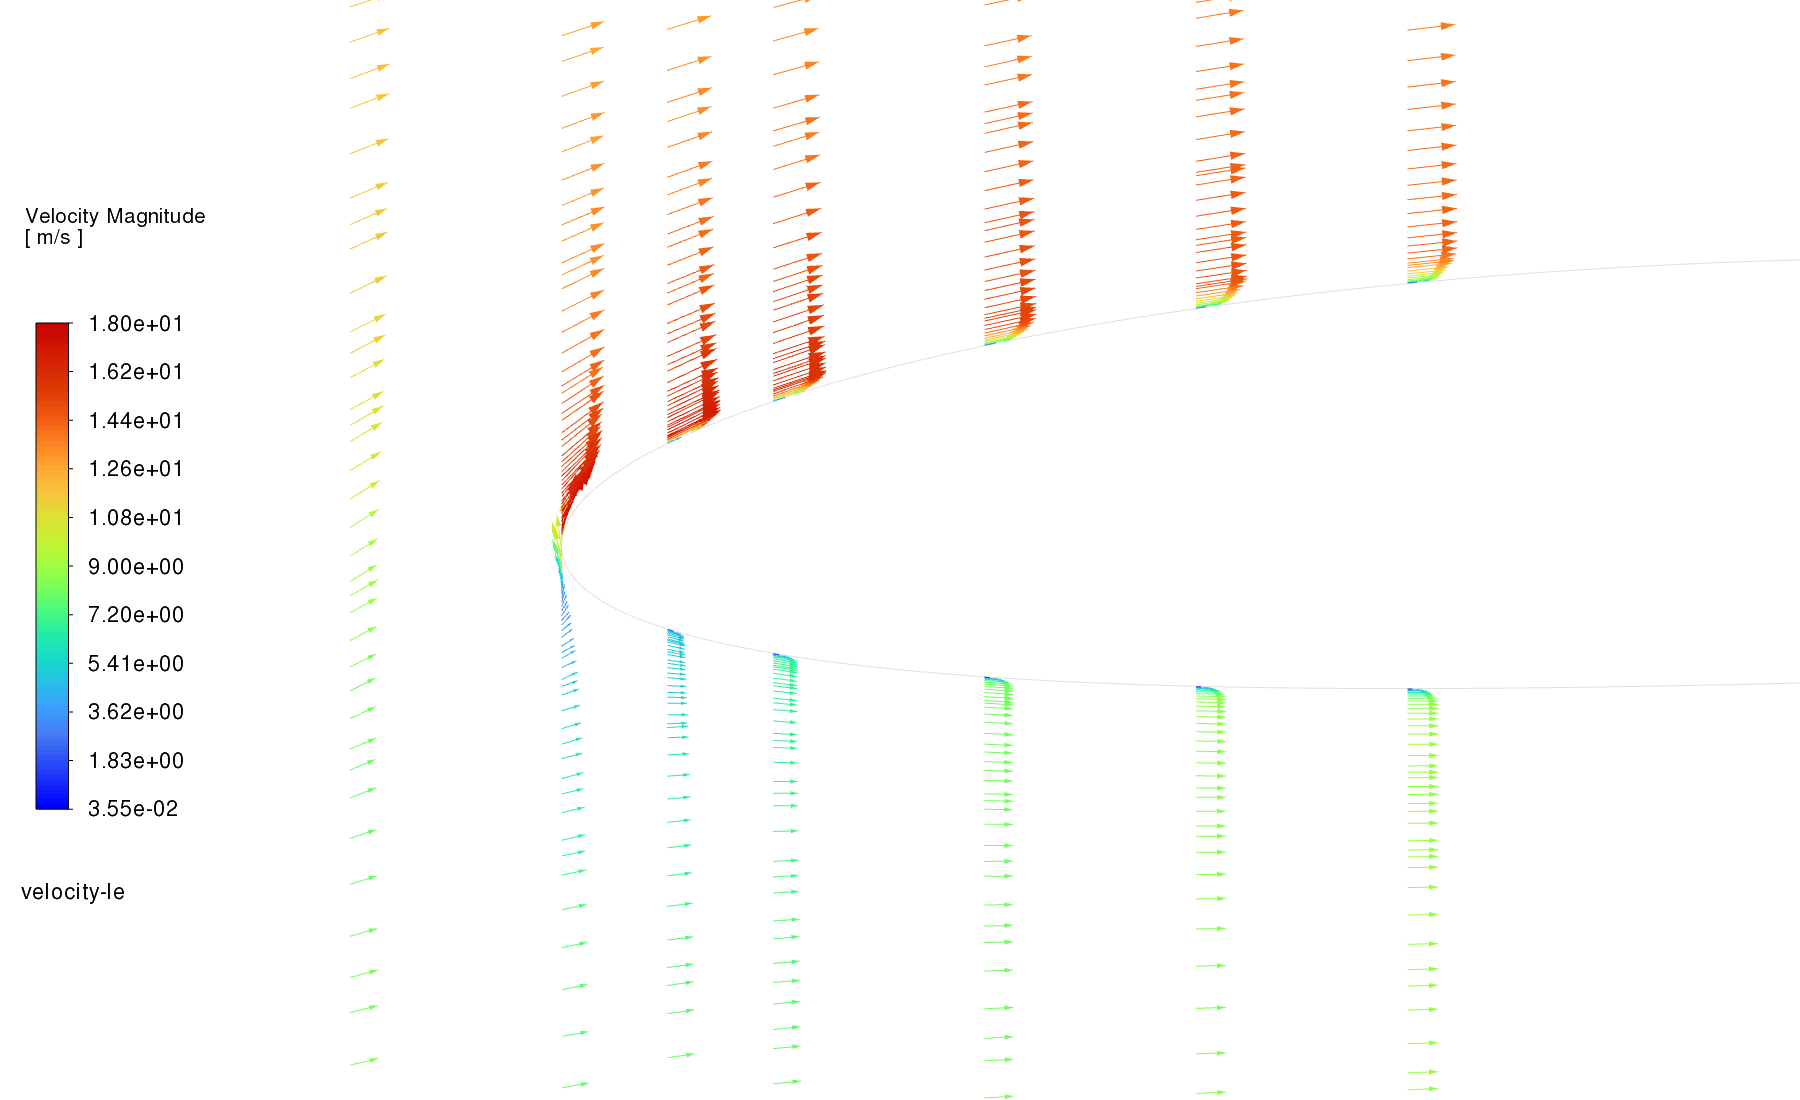
\includegraphics[width=0.85\linewidth]{fig4_quiver_le_aoa6.png}
\caption{Velocity vectors near the leading edge at $\alpha=6^\circ$, on vertical lines at $x=-0.05$, $0$, $0.025$, $0.05$, $0.1$, $0.15$ and $0.2$~m. Over the upper surface the air speeds up to about $18$~m/s, while below it stays between $4$ and $8$~m/s. Very close to the wall the arrows shrink to zero, that is the boundary layer.}
\label{fig:le}
\end{figure}

\begin{figure}[H]
\centering
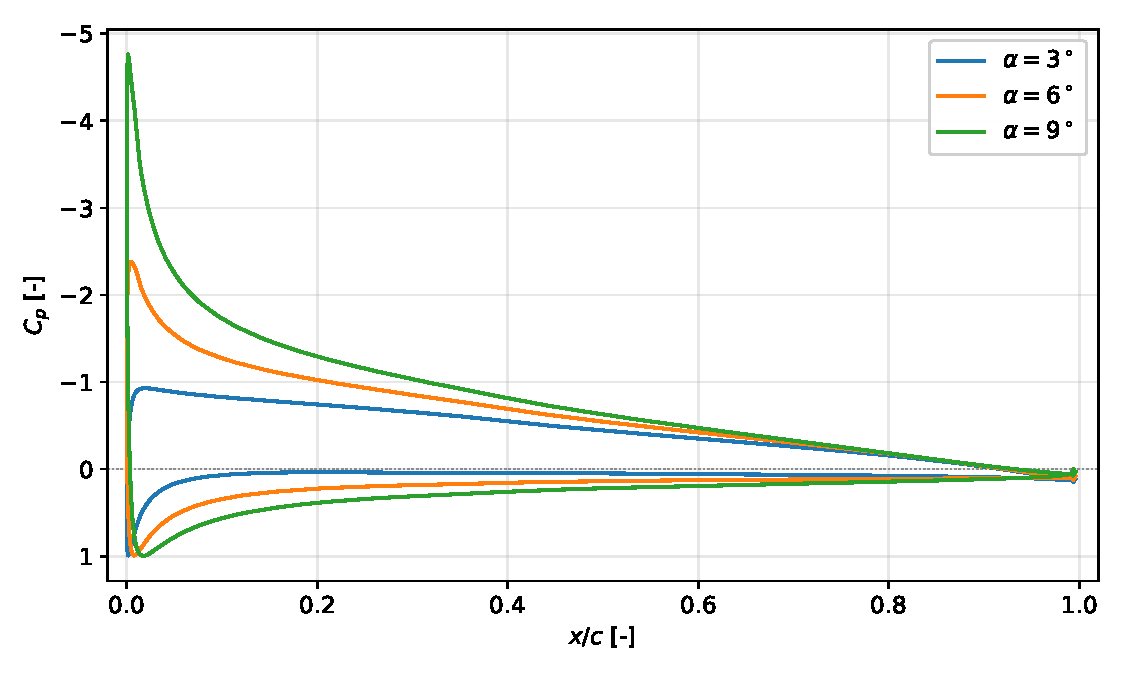
\includegraphics[width=0.85\linewidth]{fig5_cp_aoa3_6_9.pdf}
\caption{Pressure coefficient along the airfoil surface for $\alpha=3^\circ$, $6^\circ$ and $9^\circ$ (inverted $C_p$ axis, so the upper branch is the upper surface). The suction peak near the leading edge gets much stronger with the angle ($C_p\simeq-0.93$, $-2.38$ and $-4.76$). The area between the two branches grows with it, and so does the lift.}
\label{fig:cp}
\end{figure}

\begin{figure}[H]
\centering
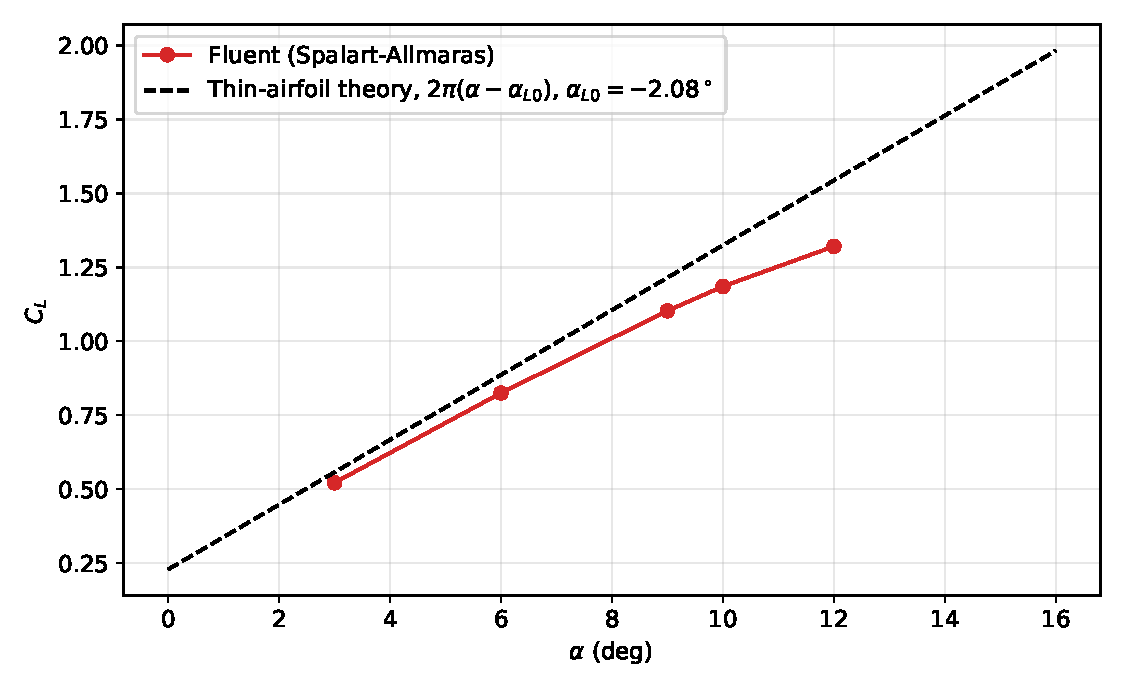
\includegraphics[width=0.85\linewidth]{fig6_cl_vs_aoa.pdf}
\caption{Lift coefficient from Fluent ($C_L=0.521$, $0.825$, $1.103$, $1.185$ and $1.321$ at $3^\circ$, $6^\circ$, $9^\circ$, $10^\circ$ and $12^\circ$) compared with thin-airfoil theory, $C_L=2\pi(\alpha-\alpha_{L0})$ with $\alpha_{L0}=-2.08^\circ$ for the NACA 2410 camber line (Anderson, \textit{Fundamentals of Aerodynamics}, Ch.~4). At small angles our results are close to the theory ($6\%$ lower at $3^\circ$, with a slope of $0.095$ per degree against $0.110$). The gap grows with the angle and reaches $15\%$ at $12^\circ$, since the theory ignores viscosity and the boundary layer on the upper surface keeps getting thicker.}
\label{fig:cl}
\end{figure}

\textbf{Extra ($\alpha=16^\circ$, 1000 iterations).} The run converged in 258 iterations and gave $C_L=1.302$, which is lower than at $12^\circ$ ($1.321$). So somewhere past $12^\circ$ the lift stops growing: the flow on the upper surface can no longer stay attached all the way to the trailing edge, and the airfoil starts to stall.

\end{document}
